\section{问题一}
\subsection{寻找特征}
根据附件提供的编译器版本信息(https://bigsearcher.com/mirrors/gcc/releases/),我们综合考量了各版本的使用情况和差异程度,选择了以下五个GCC版本作为识别对象:“8.4.0”、“10.2.0”、“11.3.0”、“12.2.0”和“13.2.0”。将程序源代码1分别由这五个版本的GCC编译器进行编译,生成对应的五个汇编文件。
我们利用VS Code自带的文本比较工具,对这五个汇编文件进行两两比对。VS Code的文本比较工具主要是基于‘Myers diff’算法实现,该算法是由Eugene Myers在1986年提出的一种广泛使用的最短编辑距离算法,专门用于计算两个序列(例如文本文件的行或字符)之间的最小修改步骤(插入、删除、替换)。
\begin{table}[H]
\caption{\textbf{Example 1}}%标题
\centering%把表居中
\begin{tabular}{l|l|l}%三列,内容全部居中

\toprule%第一道横线
\multicolumn{1}{c}{line} & \multicolumn{1}{c}{8.4.0} & \multicolumn{1}{c}{10.2.0} \\
\midrule%第二道横线 
1 &movl	252(\%rbp), \textcolor{red}{\%eax}&movl	252(\%rbp), \textcolor{blue}{\%edx} \\
  2 &\textcolor{red}{movslq	\%edx, \%rdx}&\textcolor{blue}{cltq}\\
3 &salq	\$4, \textcolor{red}{\%rdx}&salq	\$4, \textcolor{blue}{\%rax}\\
4 &leaq	272(\%rbp), \%rbx&leaq	272(\%rbp), \%rbx\\
5 &addq	\%rbx, \textcolor{red}{\%rdx}&addq	\%rbx, \textcolor{blue}{\%rax}\\
6 &subq	\$160, \textcolor{red}{\%rdx}&subq	\$160, \textcolor{blue}{\%rax}\\
7 &movl	\textcolor{red}{(\%rdx)}, \textcolor{red}{\%edx}&movl	\textcolor{blue}{(\%rax)}, \textcolor{blue}{\%eax}\\
8 &subl	\textcolor{red}{\%edx}, \textcolor{red}{\%eax}&subl	\textcolor{blue}{\%eax}, \textcolor{blue}{\%edx} \\
\bottomrule%第三道横线
\end{tabular}
\end{table}



表1展示了由'8.4.0'和'10.2.0'版本的GCC编译器生成的汇编文件中的部分差异。从表中可以看出,主要差异集中在操作码和寄存器的使用上。因此,我们计划提取汇编文件中的操作码和寄存器的数量。此外,考虑到某些可能的关联特性,如操作码与寄存器、寄存器与寄存器之间的关系,我们还将提取Bigram的数量。其中Bigram(2-gram)是指连续两个词或字符的组合,例如 "I am a student" 的 bigram 为 ['I am', 'am a', 'a student']。
\begin{figure}
    \centering
    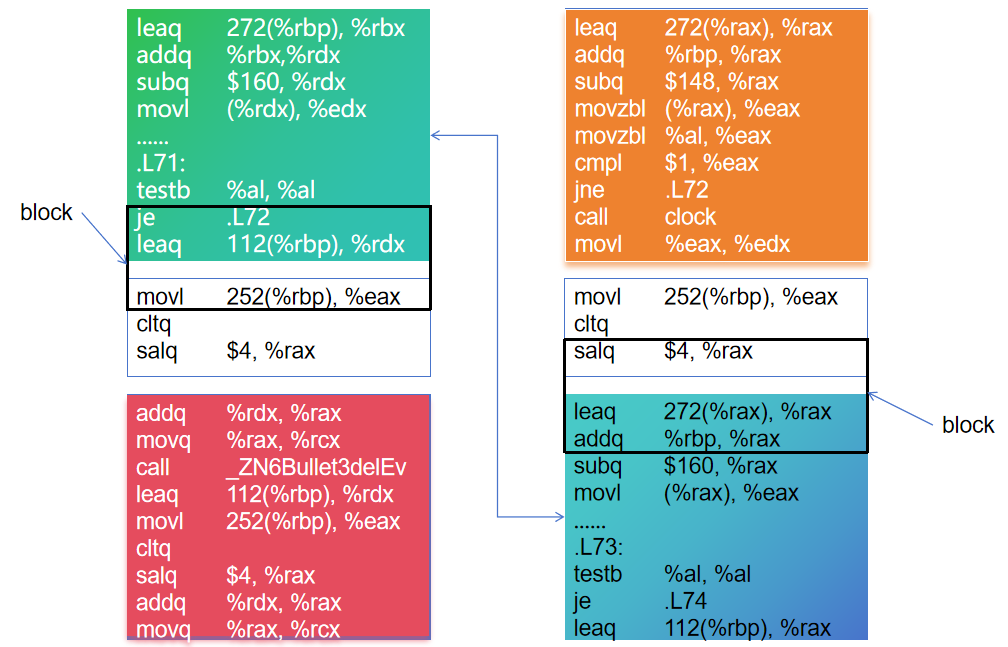
\includegraphics[width=1\linewidth]{block.png}
    \caption{Enter Caption}
    \label{fig:enter-label}
\end{figure}


  图1展示了由'10.2.0'和'12.2.0'版本的GCC编译器生成的汇编文件中的部分差异。从图中可以看出,主要差异体现在汇编代码块的位置调度上。为了捕捉这种位置特征,我们计划提取block的数量。block定义为连续的汇编指令组合,经过实验验证,我们选择连续4条汇编指令的组合效果最佳。

  综上所述,我们将提取操作码、寄存器、Bigram与block数量作为一个汇编文件的特征属性。

  \subsection{提取特征}
  对汇编文件进行特征提取之前,为了获取更加泛化有效的特征,我们对其做了一些预处理。
  
  例如,在8.4.0版本GCC编译器生成的汇编文件中,指令'movl \$98, \%eax'与'movl \$1, \%eax'都表示将一个立即数移动到寄存器\%eax中,随后寄存器中的数值即为该立即数。因此,我们将汇编文件中的所有立即数统一替换为\$0,替换后的汇编指令形如'movl \$0, \%eax'。对于指令'movl -12(\%rbp), \%eax'与'movl -20(\%rbp), \%eax',两者都表示将位于基址寄存器\%rbp偏移一定字节的内存地址中的32位数据读取到寄存器\%eax中。因此,我们统一将这些指令中的偏移量删除,替换后的汇编指令形如'movl (\%rbp), \%eax'。

  通过上述方法对汇编文件进行预处理,我们在保持其基本语义完整的前提下,能够更加有效地提取出更多相关的特征。具体来说,这些预处理步骤不仅规范了汇编指令的表示形式,还减少了特征的多样性,使得后续的特征提取和分析更加精准和高效。这种预处理方式有助于在特征选择和模型训练过程中,突出重要的特征关联,同时避免因不必要的语法差异而带来的干扰,从而提升模型的整体表现和分析的准确性。

  我们将对生成的五个汇编文件进行特征提取,最终获得的数据规模为5*428,这意味着每个汇编文件包含428个特征。由于特征维度较大,为了便于分析和展示,我们将选择前50个特征数据,并使用热力图进行可视化。通过这种方式,我们可以更直观地观察和比较各汇编文件在这些特征维度上的差异和相似性,从而为后续的数据分析提供有价值的参考。
  \begin{figure}
      \centering
      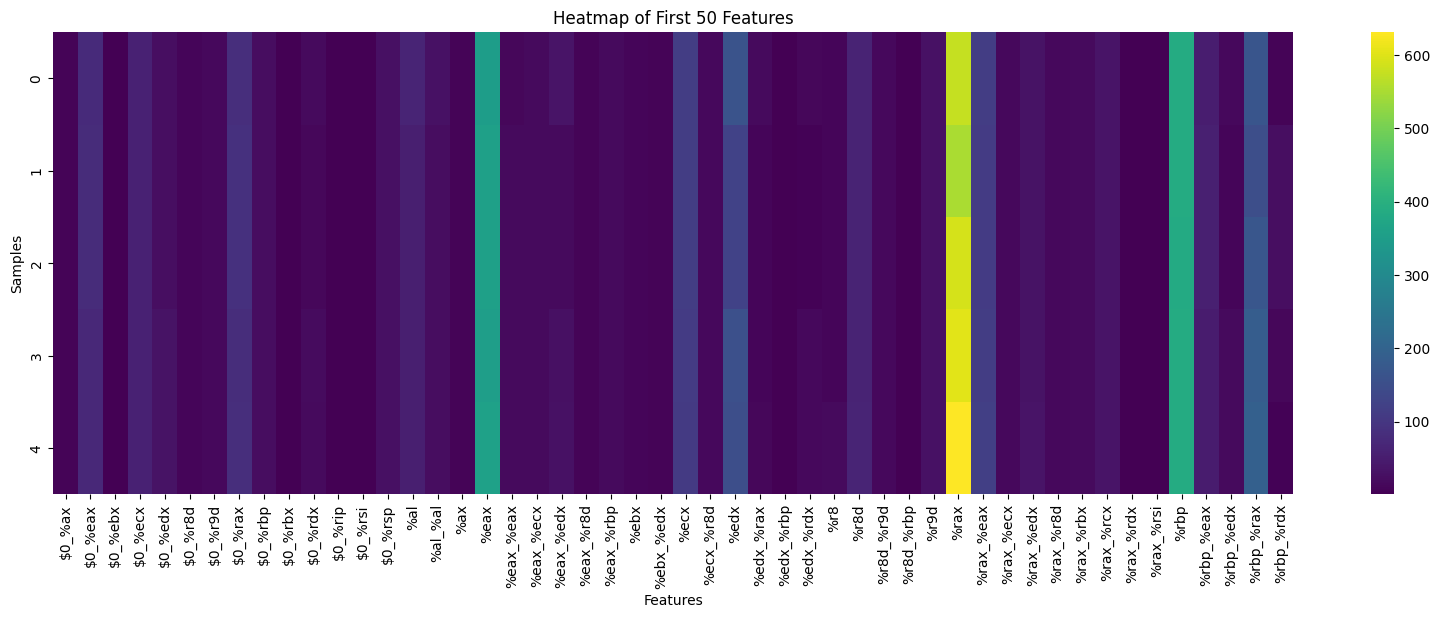
\includegraphics[width=1\linewidth]{same.png}
      \caption{Enter Caption}
      \label{fig:enter-label}
  \end{figure}


从图2可以看出,五个汇编文件在某些特征维度上的取值大致相同。鉴于此,我们决定对数据进行降维处理,将这些取值相同的特征去除。这样做有两个主要原因:一方面,减少特征维度可以降低模型的计算复杂度,简化模型的训练过程;另一方面,取值相同的特征对我们后续的版本判别并无实际帮助。因此,在降维之后,我们最终获得了规模为5*89的数据集,这意味着共有339个特征的取值是相同的,并已被剔除。
\begin{table}[H]
\caption{\textbf{Example 1}}%标题
\centering%把表居中
\begin{tabular}{lccccc}%三列,内容全部居中
\toprule%第一道横线
 feature\_name&8.4.0 & 10.2.0 & 11.3.0 & 12.2.0 & 13.2.0 \\ 
\midrule%第二道横线 
\$0\_\%eax&77&78&78&72&72 \\
\$0\_\%edx&25 & 25 & 25 & 31 & 31 \\
\$0\_\%rax&84 & 89 & 89 & 80 & 84 \\
\$0\_\%rdx&17 & 12 & 12 & 19 & 17 \\
\%al2 & 64 & 55 & 55 & 55&55 \\
...&... & ... & ... & ... & ... \\
testb&30 & 21 & 21 & 21 & 21 \\
testb\_\%al&30 & 21 & 21 & 21 & 21 \\
testb\_je\_leaq&9 & 8 & 8 & 8 & 8 \\
testl&2 & 6 & 6 & 6 & 6 \\
testl\_\%eax&2 & 6 & 6 & 6 & 6 \\
\bottomrule%第三道横线
\end{tabular}
\end{table}
   
